\section{Evolution}
In this section, we will be using the different luminosity functions from the previous section to calculate the evolution of the different classes of AGNs. 
By understanding these trends one can start understanding the nature of these objects, when and \colorbox{BurntOrange}{possibly how} they are created, and the amount of energy they release into the Universe. 

%By looking at the different trends for the different type of distributions one can observe the evolution and energy distribution of the different classes of AGNs. 


 


\subsection{Luminosity distribution}
 
For the different classes discussed one can integrate the differential luminosity function over redshift to retrieve the Luminosity distribution of each 
object. This distribution highlights the difference in emitting power and therefore is important for us to be able to distinguish the most powerful 
sources and their prevalence, and also any trends that might be interesting. One calculates the Luminosity density by multiplying the class-specific luminosity
function with the differential comoving volume and integrating over the relevant redshift bin. 
%that the evolution beyond the given luminosity range is not known and therefore the distribution is not complete. And deducing continued evolution
%can be done but must be taken with a grain of salt. The number of objects these functions are built upon are not very numberous and therefore
%the error bars are quite large, especially in the edges. 

The luminosity distribution is given as


\begin{equation}
    \frac{dN(L)}{dL} = \int_{z_{\text{min}}}^{z_{\text{max}}} \frac{\Psi(L, V(z))}{dL} \frac{dV(z)}{dz} dz
\end{equation}

Here, $z_{\rm min}$ and $z_{\rm max}$ are the limits of the redshift bin. By separating it into
bins of redshift one can assess how the class varies with redshift, and how a change in redshift would change the slope/trend of the distribution.  
%It is important to note 

\begin{figure}
    \centering
    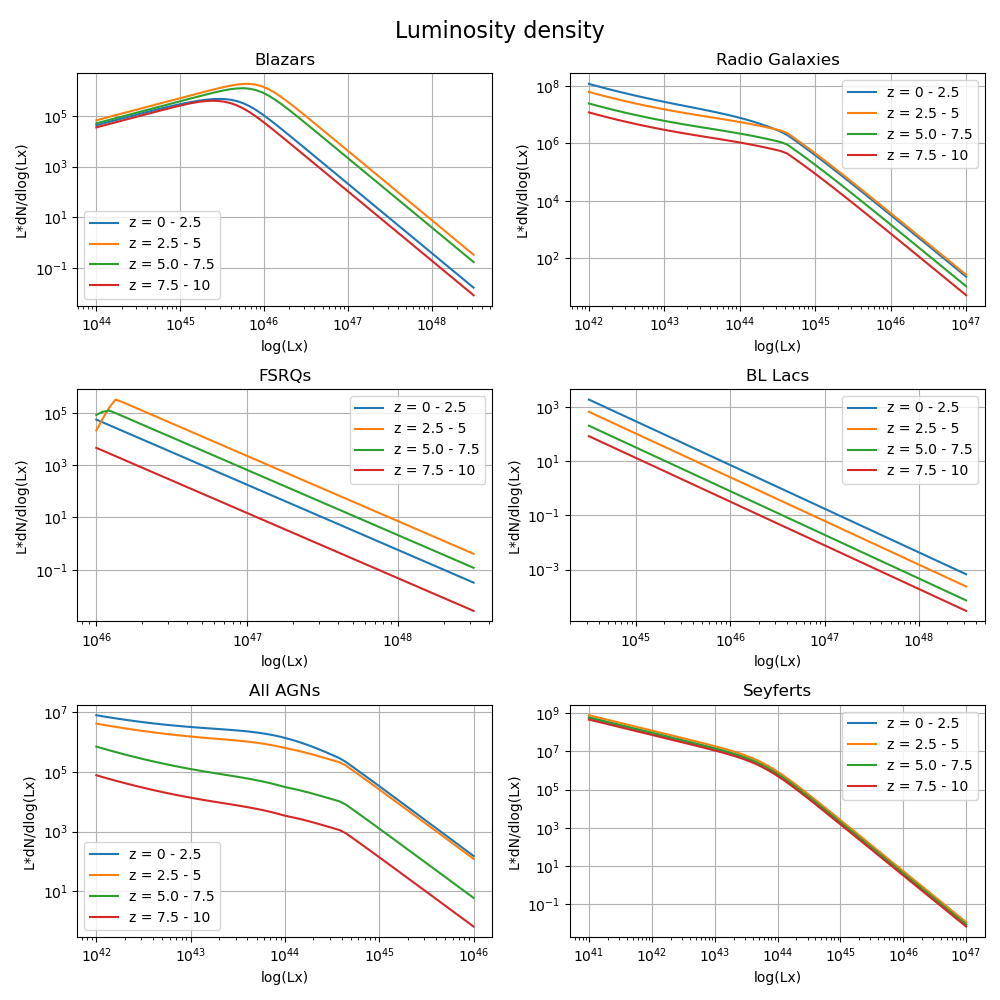
\includegraphics[width = \textwidth]{new_plots/Luminosity density.png}
    \caption{Luminosity density for the  different classes of AGNs. The different classes are defined in the title as well as the chosen LF model.}
    \label{fig:LD}
\end{figure}


In figure \ref{fig:LD} one can see the luminosity density for the six different luminosity functions. The distribution is 
separated into four bins of redshift ($0<z<2,2<z<4,4<z<6,6<z<8$). %
%This is done to illuminate the evolution of the different classes at different epochs
The most interesting feature of these distributions is the difference between the break luminosity between jet-dominated classes such as Blazars and non-jet-dominated classes such as radio galaxies and Seyferts.
For the jet-dominated ones the luminosity distribution breaks at a certain point and decreases on both sides. The only exception to this is the BL Lacs which are represented as a simple power law and therefore have no
break point in their distribution. With the inclusion of more BL Lacs in future data sets it would be interesting to see if this is still the case. %The reason for the use of a single powerlaw for the BL Lacs is namly due to the lack of observations.  
The breakpoint for Blazars and FSRQs indicates some preferred 
luminosity in which one finds the most sources. This preferred luminosity also seems consistent with different epochs. To investigate this preferred energy range one could investigate different optical bands and see if the same trend is observed. 
In \cite{Narumoto_2006} they also discuss the luminosity function for Blazars but in the gamma ray band. The evolution function they use is a luminosity dependent density evolution similar to our radio galaxies and CTN AGNs. They also find a peak in the luminosity distribution, this time at a higher luminosity than the one found here.
Therefore, it could be that there is a distribution of Blazars around a certain total luminosity since one sees this trend in the x-ray and gamma ray band. 
This is not necessarily true, and one should investigate the surveys used to see the correlation between x-ray and gamma ray luminosity. \colorbox{BurntOrange}{ From the unified model of AGN one would not expect this correlation to be negative due to the different emitting regions.}
%If so it might be explained by the production of the jet and its relation to the necessary accretion rate.
%An explanation of this preferred luminosity can with some assumptions be tied to the "Blazar sequence" and idea that Blazar luminosity is strongly tied to the synchrotron peak frequency of electrons

%In \cite{Ajello_2009} where these LFs are taken from they also highlight the flattening of the luminosity distribution for the Blazar population at lower energies. This flattening is also seen here and is attributed to 
%the beaming of the x-rays from the jet.  
%An interesting point brought up in \cite{Ajello_2009} is the effect of beaming of X-rays for Blazars. This effect flattens the XLF for lower luminositie. 


For the non-jet-dominated classes, one sees an increase in numbers towards lower energies, but at some specific luminosity radio galaxies and CTN AGN introduce a break. The break luminosity is very interesting and differentiate itself 
from jet-dominated AGN since it seems to show 
a breaking point where the creation of more powerful sources becomes significantly harder and therefore less numerous. 
%The increase in x-ray luminosity is tightly connected to the amount of accretion onto the black hole and therefore a breakpoint in the energy production of similar sources is very interesting.
This breakpoint is also varying based on the redshift bin, where for higher redshift, the break is more sudden. For the Seyferts that have no evolution factor there is no distinction between lower or higher redshift.
Any change in the slope of a power-law is cause for investigation since it seems to indicate some change in possibly the structure of the sources. The softening of the break depending on redshift 
might indicate that this break is not as sudden as one would assume looking at higher redshift objects, but the change in slope index is still observed. 
The different interpretation of the luminosity distribution of these objects is fascinating and further study could illuminate why one would observe this difference, and if it is an effect of the sources, our observation of them or not an effect at all. One notes these different reasons because the author of this paper has not found any explanation to why the number of our sources suddenly drop at a certain luminosity. 
%Another interesting point of further study would be to understand the change in slope index for radio galaxies and CTN AGN. 

%The redshift bins for the Blazar population show a very interesting trend. The amount of Blazars at lower redshift seems to not change but passed the break point the total number of Blazars becomes redshift dependent, where there is a big difference between the middle epochs and the others. 
%This is also seen for the FSRQs, but the break luminosity is met with a much steeper decline. For Bl lacs, the redshift bins show a different trend. Here the number of sources is only increasing with redshift. 


\begin{figure}[H]
    \centering
    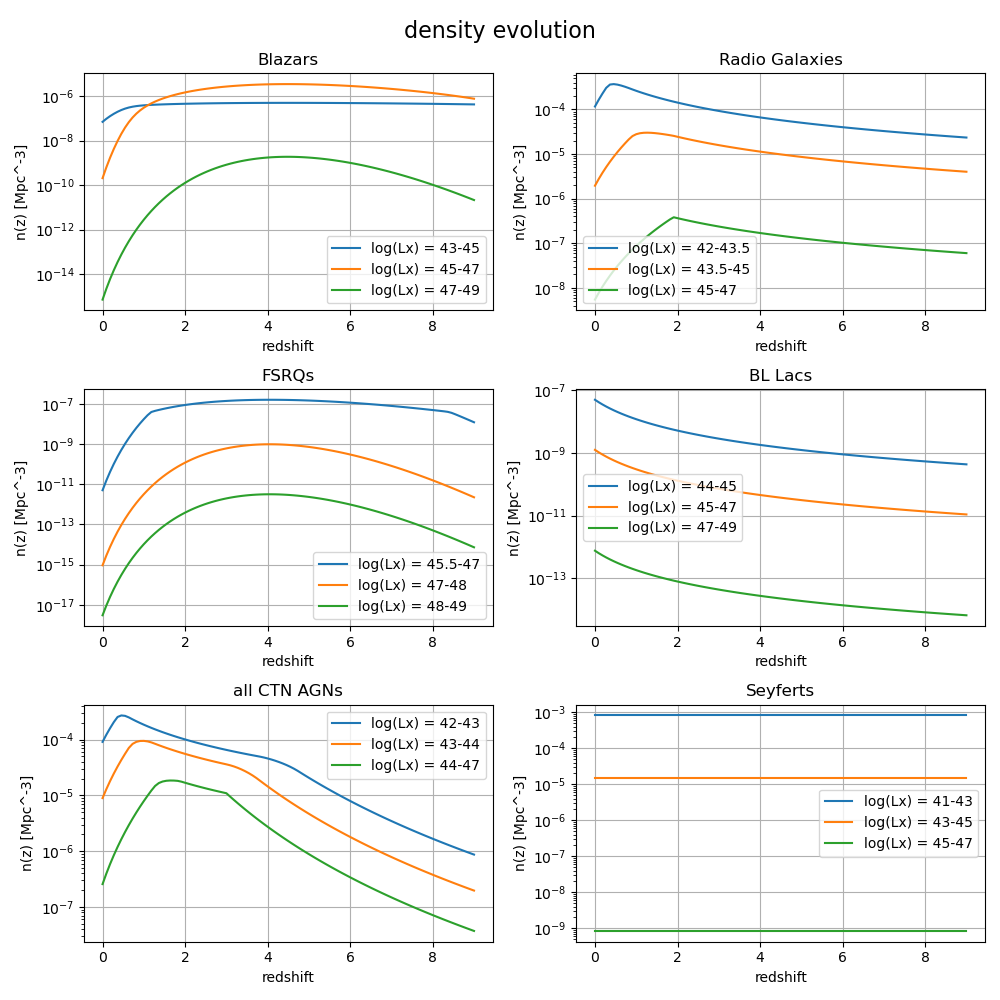
\includegraphics[width = \textwidth]{new_plots/Redshift density evolution.png}
    \caption{Density distribution for the four different classes of AGNs. The different classes are defined in the title as well as the chosen LF model.}
    \label{fig:DD}
\end{figure}



\subsection{Density distribution}

In addition to the luminosity distribution one can also calculate the number density of the different classes of AGNs. This is done by integrating the
differential luminosity function over luminosity. This will illuminate the evolution in time, or more precisely in redshift of the different classes. The integral is given as

\begin{equation}
    n(z) =\frac{N(z)}{V(z)} =  \int_{L_{\text{min}}}^{L_{\text{max}}} \frac{\Psi(L, V(z))}{dL} dL
\end{equation}

Here again, we separate into luminosity bins to see the evolution of different parts of the luminosity distribution, most notably to see the difference before and after the break luminosity for most classes. 
The results can be seen in figure \ref*{fig:DD}






%\begin{figure}
%    \centering
%    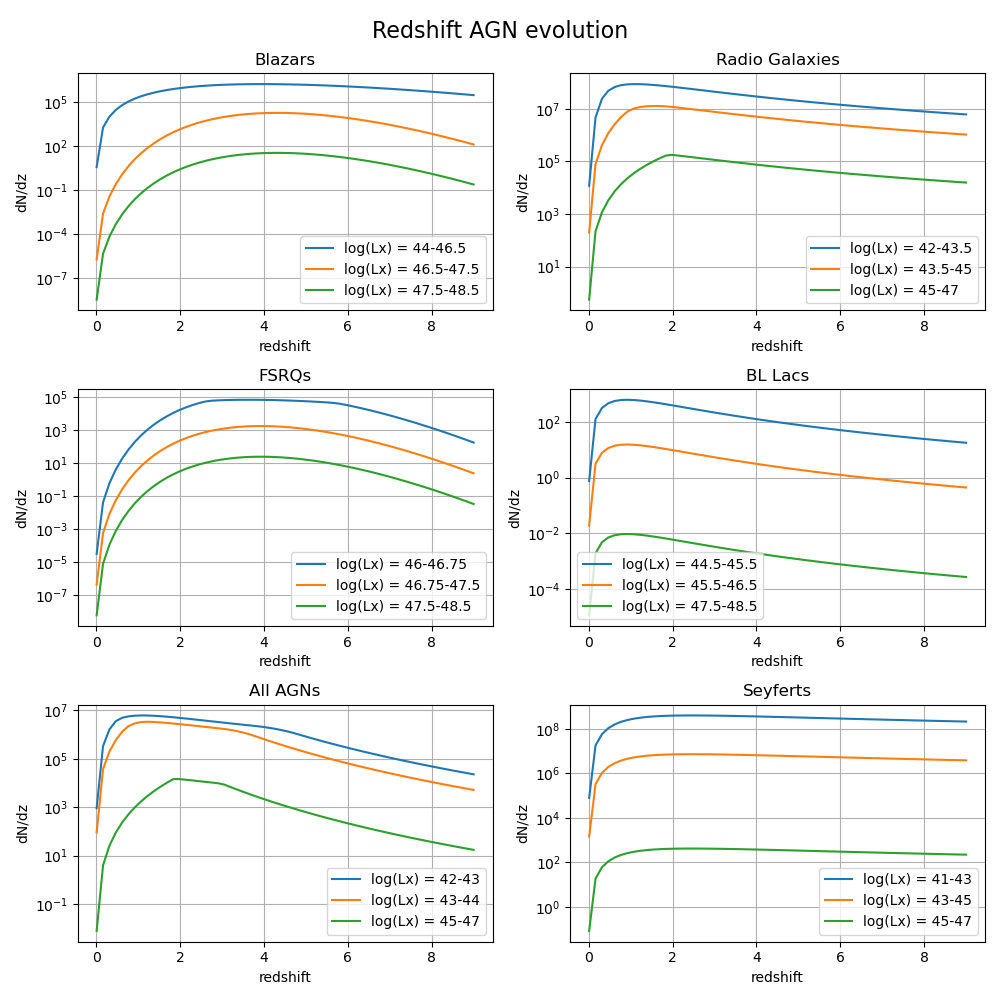
\includegraphics[width = \textwidth]{new_plots/Redshift AGN evolution.png}
%    \caption{Number evolution in terms of redshift for the four different classes of AGNs. The different classes are defined in the title as well as the chosen LF model.}
%    \label{fig:ND}
%\end{figure}


The density evolution of these objects is very interesting information due to it being closely tied to galaxy evolution. The evolution of Blazars and FSRQs differentiate themselves significantly from the other classes in figure \ref*{fig:DD}
where both FSRQs and Blazars have a positive evolution with a peak in density around redshift $z=5$. The total counterpart to this is the third class of jet-dominated AGN, the Bl Lacs. Here one sees a negative evolution with 
an increase in density in the more recent epochs. In a paper by \cite{Garofalo_2019} he talks about the different evolutionary paths that generate the respective classes of Bl lacs and FSRQs which could be the origin of this discrepancy. 
While both classes belong to the parent class of Blazars the evolutionary path of FSRQs is thought to come from FRII radio galaxies while the evolutionary path of BL Lacs is from FRI radio galaxies. As mentioned in section \ref*{sec:jets} the difference between FRI and FRII jets is thought to be the accretion efficiency. 
In addition to this a paper by \cite{Wei-Hao_2003} which studied the correlation between accretion rates and bolometric luminosity mentions that the nature of the central black hole and its rotation will have an effect on the accretion rate. Drawing from this one could indicate that the difference in evolution stems from the different evolutionary paths of their central engine, Kerr black hole or not.  
This is for the time being not an accepted explanation and still a topic of debate. 
Another try to explain how accretion efficiency is related to the central engine is in \cite{Raimundo_2012} where they discuss a finding that showed the efficiency of the accretion being proportional to the mass of the black hole.  
More precisely they found this relation: $\eta \propto M^{0.5}$. Although this could help explain our density evolution of FSRQs and Bl Lacs by allowing FSRQs to host bigger black holes they also mentioned that this effect might be an artifact of the parameter space used. 
On the other hand one could also try to look at the evolution of material that can be accreted around the central black hole to possibly start unraveling the different evolutionary paths.
From this it is only reasonable to conclude that this difference in evolution is captivating and is prone to an interesting answer. 


For the Blazar population, one notices the same trend as for the luminosity distribution. The luminosity bin before the break luminosity stays more constant than the ones after the break. The reason for such an evolution 
would likely be tied to the same mechanism driving Bl lacs and FSRQs. Due to the decline of FSRQs, one should also expect the
higher-end luminosity of Blazars to follow.

For the non-jet-dominated AGNs, one finds a different story. Here the redshift peak, if any, is at around $z=0.3$ where the peak is dependent on the luminosity bin. Lower luminosity AGN peaks at lower redshift. Therefore, the trend of density 
seems to be going toward lower-power radio galaxies and Compton-thin AGNs. 
What is very interesting is comparing this evolution to 
the evolution of star formation. From \cite{Madau_2014} the star formation rate peaks at around 3.5 billion years after the Big Bang, 
or around redshift $z= 1.9$. This is in stark contrast to our sources where only the most luminous radio galaxies and Compton thin AGNs peak at this redshift. 
The star formation rate then places itself in between the two peaks between jet-dominated and non-jet-dominated AGNs which opens up for interpretation. 
%This is very interesting since then the presence of efficient accreting AGN such as our FSRQs would have been more numerous before the peak of star formation. 
%And on the opposite side our CTN AGNs peak later.  


\subsection{Expected luminosity}
\label{sec:Expt_lum}
From the luminosity function, one can also calculate the expected luminosity of a source class at different redshifts. This is important since it will directly relate to the 
power injection of the different epochs and from this one can calculate an expected emissivity of the different classes of AGNs. 
The expected luminosity of each group can be calculated with the following formula

\begin{equation}
    \langle L \rangle = \frac{\int_{L_{\text{min}}}^{L_{\text{max}}} L \frac{\Psi(L, V(z))}{dL} \frac{dV(z)}{dz} dL}{\int_{L_{\text{min}}}^{L_{\text{max}}} \frac{\Psi(L, V(z))}{dL} \frac{dV(z)}{dz} dL}
\end{equation}

furthermore, the emissivity is given as


\begin{equation}
     \epsilon  = \int_{L_{\text{min}}}^{L_{\text{max}}} L \frac{\Psi(L, V(z))}{dL} \frac{dV(z)}{dz} dL
\end{equation}

The different luminosity ranges are the same as before and are given in table \ref{tab:lum_range}. The results are shown in figure \ref{fig:EL}.

\begin{figure}
    \centering
    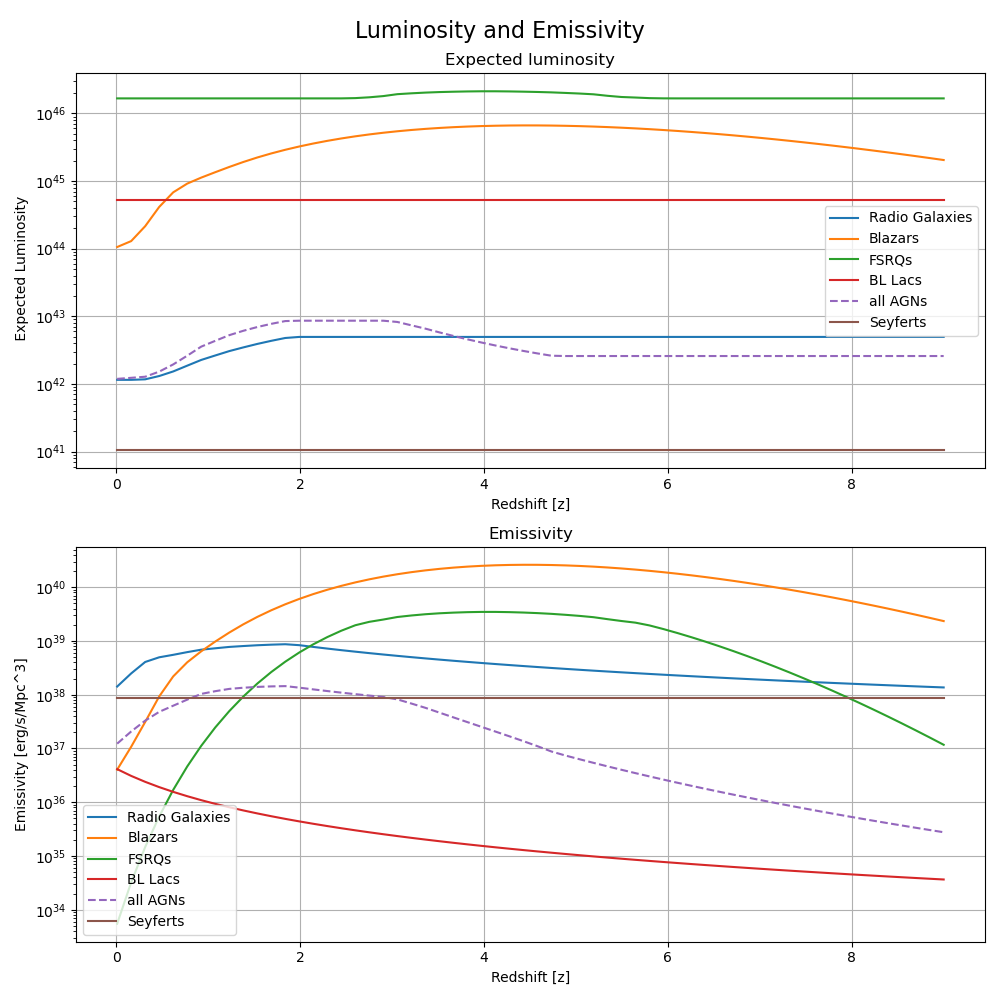
\includegraphics[width = 0.8\textwidth]{new_plots/Luminosity and Emissivity.png}
    \caption{Expected luminosity and emissivity for the four different classes of AGNs. The different classes are defined in the title as well as the chosen LF model.}
    \label{fig:EL}
\end{figure}



The expected luminosity is shown at the top in figure \ref*{fig:EL} where it shows the expected power output of the different classes. Here one sees that FSRQs are indeed the most luminous AGN and 
that they represent some of the most luminous objects in the Universe.
The expected luminosity also shows the evolutionary trend of Blazars where they are now tending towards lower average luminosity. 
All classes remain fairly constant, but radio galaxies and CTN AGNs both have a decline in expected luminosity after the star formation peak at $z=1.9$. This could be inferred from figure \ref*{fig:DD} but is more clearly seen here.
%The constancy of most objects across redshifts is comforting since it means that one could use a general model for any of the objects at any redshift without needing to account for the redshift. 
%This is not the case for the Blazars but since they are a combination of different objects any general model would be hard to find. On the other hand, any model for FSRQs and Bl lacs would not need to account for redshift and the varying parameters that come with that. 
%An important point to remeber is that this luminoisty is directly tied to the x-ray production of these sources. Therefore the expected luminoisty also shows us that 
%jet-dominated AGN produce more x-rays than non-jet-dominated AGN. This is not suprising but it is a indcication that these x-rays are not only produced in the hot corona, but also in the jet. 
%While for all compton thin AGNs one would expect the x-ray luminosity to be dominated by the hot corona.

The emissivity of each class as a function of redshift is shown in figure \ref*{fig:EL} at the bottom. Here it shows a change in dominance between Blazars and our CTN and radio galaxies.
%The change in dominance happens around redshift $z=1$ and is a result of the different evolution of the different classes.
This change that happens around redshift $z=1$ is a result of the different evolutionary paths of our sources seen in figure \ref*{fig:DD} and should affect the diffuse astrophysical flux of UHECRs and neutrinos. 
Due to the different orientations of the sources one should expect them to create UHECRs and neutrinos differently. From this any decline in emissivity of for example Blazars would separate the expected flux of neutrinos and UHECRs if they are produces in the same source. This is due to the energy loss mechanisms 
discussed in section \ref{sec:emmisivity}. In order to test this one would need a way of correlating the production of neutrinos with UHECRs, and this requires to model the different ways of not only accelerating particles but also the direction of acceleration. 
Two possible ways of accelerating particles which compliments the different classes discussed in this report is the Blandford-Znajek process which produces jets, and outflow mechanics which can in theory take any direction but are usually discussed as outflows into the plane of the host galaxy.
For jet-dominated AGNs the most accepted theory of energy extraction from rotating black holes is discussed in \cite{Blandford_1977}. This method of acceleration which is produced by ordered electric fields drives the accelerated particles into jets. One cares about this since any emission of particles especially neutrinos would therefore be highly pointed and one would only expect 
AGNs with a jet pointed in our line of site to produce neutrinos we would detect. 
The method of outflows discussed in \cite{Laha_2021} is another way of accelerating particles \colorbox{BurntOrange}{and is akin of reconnection events that happen in the sun}. The problem one faces here is 
therefore the uncertainty of accelerating our particles enough. The mechanism of outflow is not certain enough to produce the highest energy UHECRs and neutrinos. The orientation of these outflows can be also be difficult to determine therefore it becomes harder to use these outflows as consistent methods of generating our desired particles.
These different ways of accelerating our particles are important to consider later when talking about the diffuse flux of UHECRs and neutrinos since they would be quite dependent on the class of AGN.


 \colorbox{BurntOrange}{A note for Foteini: The last paragraph is in my opinion important, but I find it awkwardly placed, and} - \\
 \colorbox{BurntOrange}{I feel like I do not know enough to keep it in, please correct me if I have written anything wrong or weird.}
%The emissivity is a good indicator of what objects might dominate the different epochs, and it is clear that at higher redshift $z>2$ our jet-dominated AGNs are the most powerful emitters of x-rays. 
%An interesting point is how this increase in emissivity of different classes of AGNs would affect the outflow mechanism of the AGNs and how this would affect the surrounding galaxy. In \cite{Laha_2021}
%they talk about the open questions regarding the outflow mechanism of AGNs and their feedback mechanism with their host galaxy. To add to these open questions one could ask how the change in x-ray emissivity in the different classes of AGNs would affect the same mechanisms.

